\chapter{Rendszertervezés és követelmények}

\section{Rendszeráttekintés}
Az autonóm fegyverrendszer fejlesztése során egy komplex mechatronikai rendszert kellett megvalósítani, amely több különálló modul együttműködését biztosítja. A rendszer fő komponensei közé tartozik a \textsl{mechanikai szerkezet}, az \textsl{elektronikai hardver}, az \textsl{érzékelők}, a \textsl{vezérlő egység}, valamint a \textsl{szoftveres háttér}. Ezek együttesen biztosítják a rendszer autonóm és manuális működését. Az alábbiakban részletes áttekintést adok a rendszer főbb elemeiről és azok feladatáról.

\subsubsection*{Mechanikai konstrukció}

A váz gyanánt tulajdonképpen egy kéttengelyes \textsl{pan-tilt} mechanizmust kellett megvalósítanom, ami felelős a fegyver stabilan tartásáért és precíz mozgásáért. A váz építőelemei zömében 3D nyomtatási technológiával készültek, ami lehetővé tette a problémák gyors kiküszöbölését, illetve a nagyfokú szabadságot a tervezés során. Ahol tudtam, kereskedelemből beszerezhető alkatrészeket használtam, például a csapágyakat és a kötőelemeket.\\

A modellt több alegységre lehet bontani a funkciójuk szerint. Van a \textsl{torony} nevezetű alösszeállítás, amely feladata a gearbox stabil befogása, illetve erre épül rá a kamera konzolja, a tár összeállítása, a fogaskerék és a lézer is. A következő a \textsl{keret}, amelybe kerülnek a torony csapágyai, illetve az elektonika egy része. Erre az elemre van erősítve a Raspberry Pi konzolja, a relé, illetve az egyik motor is. A torony alatt található a \textsl{nagy csapágyhoz }tartozó elemek, amelyeknek feladata a stabil összeköttetés biztosítása a keret és a talp között. Legalul helyet kapott a \textsl{talp}, amely magába foglalja a lábakat, illetve az azokat összefogó elem is. Ezt úgy terveztem, hogy a lábak szükség esetén cserélhetőek legyenek.

\pagebreak
\subsubsection*{Elektronikai rendszer}
Az elektronikai rendszer blokkdiagrammja a \ref{fig:system_blokkdiagram}. ábrán látható.\\

\begin{figure}[h!]
	\centering
	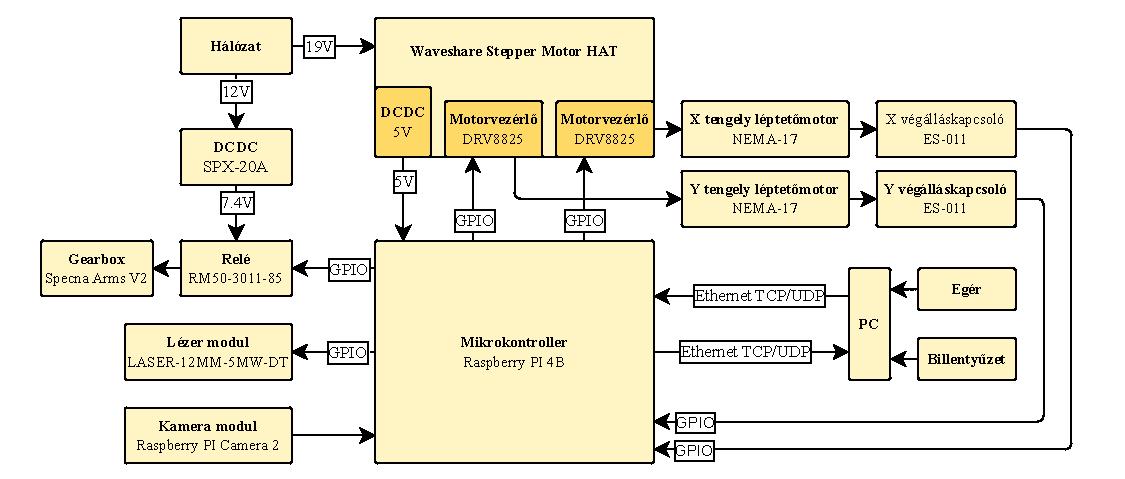
\includegraphics[width=1\linewidth]{blokkdiagram_vegleges}
	\caption{Az elektronikai rendszer blokkdiagrammja}
	\label{fig:system_blokkdiagram}
\end{figure}

Az elektronikai rendszer két fő eleme a \textsl{Raspberry Pi}, illetve a \textsl{gearbox} volt. Mivel a gearbox igen nagy áramot képes felvenni, külön tápegységgel kellett ellátnom a mikrovezérlőt illetve a golyó kilövéséért felelős elektronikát. A motorok vezérléséért egy kereskedelemben kapható, Raspberryvel kompatibilis shieldet használtam, amely jelentősen megkönnyítette a NEMA-17 típusú léptetőmotorok csatlakoztatását. A lézer diódát és szükséges szenzorokat a Raspberry Pi GPIO lábairól vezéreltem, ahogy a gearbox aktiválásáért felelős relét is. A kamera modul egy Raspberry Pi Camera V2 volt, amit a mikrovezérlőn található foglalaton keresztül tudtam elérni.\\ 

Az elektronika központi egysége természetesen a \textsl{Raspberry Pi} mikrokontroller volt, amely felelős volt a fő képfelismerő algoritmus futtatásáért, a szenzorok jeleinek feldolgozásáért, valamint a PC-vel való kommunikációért. A mikrokontroller kiegészült egy \textsl{Stepper Motor HAT}-el, amely egy kereskedelemben kapható áramkör. Megtalálható rajta két db. \textsl{DRV8825} motorvezérlő chip, illetve kiegészítő áramkörök, pl. microstep állító kapcsolók, valamint áramkorlátozó potméterek. Ezentúl helyet kapott egy 5V-os DCDC konverter, amin keresztül a Raspberry Pi-t is elláthatjuk árammal. A léptetőmotorok \textsl{NEMA-17} típusúak, és 4 tüskés csatlakozóval rendelkeznek.\\

Az elektronikai rendszerben szerepel még a \textsl{gearbox}, ami a tüzelésért felel. Mivel igen nagy áramot képes felvenni, ezért külön áramellátást terveztem a gearboxnak. Egy 12V-os szervertáp működteti, amiből egy \textsl{SPX-20A} típusú, nagy teljesítményű DCDC konverter csinál a gearbox számára optimális 7.4V-ot. Ez a kimeneti feszültség állítható, a gearbox egészen 11V-ig képes működni. A kimeneti feszültséggel tulajdonképpen a tüzelés sebességét tudjuk szabályozni. A gearbox áramellátását egy relével lehet vezérelni, amely a Raspberry Pi GPIO lábára csatlakozik.

\pagebreak

A rendszerben helyet kapott mindkét tengelyre 1-1 \textsl{végálláskapcsoló}, amelyek a fegyver kalibrálásáért felelősek. Ezek a GPIO tüskesoron csatlakoznak a mikrovezérlőhöz. Hasonlóképpen a \textsl{lézer dióda} is, amely a fegyver célzásával hivatott segíteni a felhasználót. A RAspberry Pi kamera csatlakozóján keresztül pedig beépítésre került egy \textsl{Raspberry Pi Camera 2} típusú kamera. A mikrovezérlő a rajta található \textsl{Ethernet} porton keresztül kommunikál a PC-vel.

\subsubsection*{Számítógépes vezérlés és szoftveres háttér}
A szoftver rendszere két alegységből áll, a Raspberry Pi-n \textbf{beágyazott vezérlő szoftverből}, illetve a PC-n futó \textbf{felhasználói alkalmazásból}. Mivel magát a prototípust szeretném minél jobban közelíteni a valósidejű működéshez, ezért a két alegység közötti kommunikáció sebessége kiemelkedően fontos. Ezért döntöttem úgy, hogy a Raspberry Pi az Ethernet portján keresztül csatlakozzon a PC-hez. Ez ugyan kissé megköti a fegyver mozgásterét, de nem annyira, hogy feláldozzam a kapcsolat gyorsaságát. \\

A Raspberry Pi-n futó szoftver felelős a léptetőmotorok mozgatásáért, a felhasználó parancsainak fogadásáért, a célpont felismeréséért, illetve a  kamera képének továbbításáért a PC felé. Ezeket a folyamatokat jól elkülönülő modulokra bontottam, amelyek egyszerre futnak külön szálakon. A különböző folyamatok közötti kommunikációra használtam megosztott erőforrásokat, állapotjelzőket és queue-kat. A kézi vezérlés és az automata működés között is tettem különbséget, a szoftver bizonyos részei között is megosztott változókkal lehet választani. \\

A PC-n futó szoftver felelős a Raspberry által küldött videó dekódolására, és megjelenítésére a \textsl{HUD}-on. A HUD-on szerepelnek még fontos állapotjelzők, pl. hogy éppen melyik működési módban van a rendszer, vagy hogy be van-e biztosítva a fegyver. Emellett A szoftvernek fel kell dolgozni a felhasználótól kapott parancsokat is, és tovább kel küldenie a Raspberry Pi felé. Ez a program is két külön szálon futó alegységből áll, amelyek megosztott erőforrásokkal kommunikálnak egymással. 

\pagebreak

\section{Követelmények}\label{sec:kov}


Az autonóm fegyverrendszer fejlesztése során számos követelményt kellett figyelembe venni annak érdekében, hogy a rendszer megbízhatóan, hatékonyan és biztonságosan működjön. Ezek a követelmények a rendszer mechanikai, elektronikai és szoftveres elemeire egyaránt kiterjedtek. A következő szakaszokban részletezem a legfontosabb műszaki és funkcionális követelményeket.

\subsubsection*{Mechanikai követelmények} 

A mechanikai komponensek tervezése során az alábbi követelményeknek kellett megfelelni:
\begin{list}{$\bullet$}{}
	\item \textbf{Stabilitás és pontosság:}  A fegyverrendszer mechanikai szerkezetének stabilnak és tartósnak kell lennie annak érdekében, hogy a lövések közben ne mozduljon el, és ne veszítse el a célpontot. Ugyanakkor elegendő pontosságot kell biztosítania a célpont precíz követéséhez.
	\item \textbf{Fürgeség:} A rendszernek képesnek kell lennie a fegyver gyors és pontos mozgatására a pan-tilt mechanizmus segítségével. Ennek megfelelően a szervomotoroknak kellően gyorsnak és erősnek kell lenniük ahhoz, hogy valós időben tudják követni a mozgó célpontokat.
	\item \textbf{Strapabíró konstrukció:} Habár nagy terhelés nem fogja érni, a gearboxból jöhetnek rezgések, rángások, amik esetleg problémát jelenthetnek egy alulméretezett alkatrész esetében.
\end{list}

\subsubsection*{Elektronikai követelmények}

Az elektronikai rendszer megbízható működése érdekében az alábbi követelményeknek kellett eleget tenni:

\begin{list}{$\bullet$}{}
	\item \textbf{Megfelelő teljesítmény:}  A szervomotoroknak és szenzoroknak megfelelő tápegységre van szükségük, amely stabil energiaellátást biztosít. A rendszer energiaigényét előzetesen fel kellett mérni, hogy a tápegység terhelés alatt is megfelelően működjön.
	\item \textbf{Szenzorok pontossága:} A kamerának és egyéb szenzoroknak elegendő felbontással és érzékenységgel kell rendelkezniük ahhoz, hogy képesek legyenek a célpontokat megfelelően azonosítani. A valós idejű képfeldolgozás nagy adatsebességet és megbízható szenzorjeleket igényel.
	\item \textbf{Vezérlés:} A mikrokontrollernek kellően gyorsnak kell lennie, hogy a valós idejű adatokat folyamatosan feldolgozza és a vezérlési parancsokat késlekedés nélkül végrehajtsa.
\end{list}
\pagebreak

\subsubsection*{Szoftveres követelmények}

A rendszer működéséhez szükséges szoftverfejlesztés során a következő követelményeknek kellett megfelelni:

\begin{list}{$\bullet$}{}
	\item \textbf{Valós idejű feldolgozás:}  A számítógépes látás szoftverének valós időben kell elemeznie a kamerák által közvetített adatokat, felismerve a célpontokat és kiszámítva a mozgás irányát. A célzási és lövési döntések gyors és hatékony adatfeldolgozást igényelnek.
	\item \textbf{Biztonságos működés:} A rendszernek rendelkeznie kell olyan szoftveres biztonsági funkciókkal, amelyek megakadályozzák a véletlen tüzelést. Ez magában foglalja a lövési engedélykérés mechanizmusát és a manuális vészleállítás lehetőségét.
	\item \textbf{Felhasználói interfész:} Az felhasználónak egyszerű és intuitív felhasználói felületet kellett biztosítani, amelyen keresztül könnyedén vezérelheti a rendszert, illetve áttekintheti a célpontok adatait és a kamera képét. A felületnek támogatnia kell a kézi irányítást és a lövési parancsok kiadását.
\end{list}




\subsubsection*{Funkcionális követelmények}

A rendszer teljes funkcionalitásának biztosítása érdekében a következő kritériumoknak kellett megfelelni:

\begin{list}{$\bullet$}{}
	\item \textbf{Autonóm működés:} A rendszernek képesnek kell lennie arra, hogy teljesen önállóan felismerje és kövesse a célpontokat, valamint meghozza a tüzelési döntéseket az előre meghatározott paraméterek alapján.
	\item \textbf{Manuális vezérlés:} Az autonóm működés mellett manuális vezérlési lehetőséget is kellett biztosítani az operátor számára. Ezen keresztül a felhasználó közvetlenül irányíthatja a fegyvert és manuálisan adhat lövési parancsot.
\end{list}

\subsubsection*{Biztonsági követelmények}

Az autonóm fegyverrendszerek használatával kapcsolatban különösen fontos a biztonsági követelmények teljesítése:

\begin{list}{$\bullet$}{}
	\item \textbf{Vészleállítás:} A rendszernek rendelkeznie kell egy vészleállító gombbal, amely azonnal megszakítja a fegyver működését, ha bármilyen hiba vagy vészhelyzet lép fel.
	\item \textbf{Engedélyezési mechanizmus:} A tüzelési parancs kiadása előtt a rendszernek engedélyt kell kérnie az operátortól, ezzel minimalizálva a véletlen tüzelés kockázatát.
	\item \textbf{Adatbiztonság:} A vezérlő szoftver és az operátor közötti kommunikáció titkosítva kell, hogy legyen, hogy megakadályozza a külső hozzáférést és a rendszer kompromittálását.
\end{list}

\pagebreak

\subsubsection*{Környezeti követelmények}

A rendszernek különféle környezeti feltételek között is megbízhatóan kell működnie:

\begin{list}{$\bullet$}{}
	\item \textbf{Hőmérsékleti tűréshatár:}A rendszernek képesnek kell lennie normál működésre különböző hőmérsékleti körülmények között, amelyek tipikusan a beltéri használat során fordulnak elő.
	\item \textbf{Nedvesség és porállóság:} A rendszert úgy kell megtervezni, hogy ellenálljon a kisebb por- és nedvességterhelésnek, különösen, ha kültéri használatra is szükség van.
\end{list}

Azokhoz a követelményeket, amelyekhez tudok konkrét értéket rendelni, az alábbi táblázatban gyűjtöttem össze:

\begin{table}[ht]
	\footnotesize
	\centering
	\begin{tabular}{ c l c }
		\toprule
		\textbf{Nr.} & \textbf{Követelmény}                  & \textbf{Érték} \\
		\midrule
		1.           & Szögsebesség                          & 45°/ s \\
		2.           & Valósidejűség kézi vezérlésen         & 10 ms \\
		3.           & A célpont felismerése a képbe kerülés után    & 0.5 s \\
		4.           & Vízszintes tengely mozgási tartomány  & -10°\textless{}x\textless{}75°  \\
		5.           & Függőleges tengely mozgási tartomány  & -135°\textless{}y\textless{}135° \\
		6.           & Tüzelés pontossága 5m-en, 20cm x 20cm & 80\%                             \\
		7.           & Felhasználói felület felbontása       & 640x480                          \\
		8.           & Hőállóság                             & -10°C\textless{}T\textless{}50°C \\
		\bottomrule
	\end{tabular}
	\caption{Az órajel-generátor chip órajel-kimenetei.}
	\label{tab:TabularExample}
\end{table}